%\documentclass[12pt, oneside]{report}
\documentclass[oneside,13pt]{extreport}
%\KOMAoption{fontsize}{16pt}
%\documentclass[13pt]{extarticle}  
\usepackage[ a4paper, total={155mm,232mm}, left=35mm, top=30mm,]{geometry}

\usepackage[utf8]{inputenc}
%\usepackage{mathptmx} % Times new Roman font
%\usepackage[charter]{mathdesign}
\usepackage{amsmath}
\usepackage{amssymb}
\usepackage[lined, linesnumbered, figure, longend]{algorithm2e}
\usepackage{listings}
\usepackage{nameref}
\usepackage{url}
\usepackage{imakeidx}
\usepackage{graphicx}
\usepackage{svg}
\usepackage{enumitem}
\usepackage{multirow}
\usepackage[labelsep=newline,font=sc, justification=centerlast]{caption}
\graphicspath{ {figures/} }
\usepackage{array}
\makeindex[columns=2, intoc]
\usepackage{setspace}
\usepackage[english]{babel} % for vietnamese support
\usepackage{tikz} % for drawing rectangle
\usepackage{color, colortbl}
\usetikzlibrary{calc}

\lstdefinestyle{mystyle}{
    basicstyle={\footnotesize},
    breakatwhitespace=false,         
    breaklines=true,                 
    captionpos=b,                    
    keepspaces=true,
    columns=fullflexible,
    aboveskip=1mm,
    belowskip=1mm,
    numbers=none,
    numbersep=5pt,                  
    showspaces=false,                
    showstringspaces=false,
    showtabs=false,                  
    tabsize=4
}

\lstset{style=mystyle}

\let\oldnl\nl% Store \nl in \oldnl
\newcommand{\nonl}{\renewcommand{\nl}{\let\nl\oldnl}}%
\newcommand{\B}[1]{\textbf{#1}}  %Bold
\newcommand{\I}[1]{\emph{#1}}    %Italics
\newcommand{\ws}[1]{\url{#1}}
\newcommand*\cleartoleftpage{%
  \clearpage
  \ifodd\value{page}\hbox{}\newpage\fi
}
\renewcommand{\baselinestretch}{1.5}
\definecolor{LightCyan}{rgb}{0.88,1,1}

\begin{document}

\clearpage
%%\usepackage[top= 1in, bottom= 1in, left= 1in, right= 1in]{geometry}
\begin{titlepage} 
%\cleartoleftpage
\begin{tikzpicture}[remember picture, overlay]
  \draw[line width = 1pt] ($(current page.north west) + (1in,-1in)$) rectangle ($(current page.south east) + (-1in,1in)$);
\end{tikzpicture}
%\begin{center} % Upper part of the page. The '~' is needed because \\ % only works if a paragraph has started.
%
%\includegraphics[width=0.15\textwidth]{./hyperplane_svm}~\\[1cm] \textsc{\LARGE University of Beer}\\[1.5cm] 
%\textsc{\Large Final year project}\\[0.5cm] % Title 
%\HRule \\[0.4cm] { \huge \bfseries Lager brewing techniques \\[0.4cm] } 
%\HRule \\[1.5cm] % Author and supervisor 
%\noindent \begin{minipage}[t]{0.4\textwidth} 
%\begin{flushleft} \large \emph{Author:}\\ John \textsc{Smith} \end{flushleft} \end{minipage}% 
%\begin{minipage}[t]{0.4\textwidth} \begin{flushright} \large \emph{Supervisor:} \\ Dr.~Mark \textsc{Brown} \end{flushright} \end{minipage} \vfill % Bottom of the page 
%{\large \today} \end{center} 

\begin{center}
{\fontfamily{hfbright}\selectfont
\textbf{\large UNIVERSITY OF SCIENCE \\[0.25cm]
ADVANCED PROGRAM IN COMPUTER SCIENCE}\\[1cm]

\textsf{\large Cao Dung Anh - Hoang Phuong Anh
}\\[3cm]

\textbf{\color[rgb]{0.255, 0.412, 0.882} \Large 
INCREMENTAL SVD++ FOR RECOMMENDER SYSTEMS
}
}\\[2cm]
\textbf{ \large
BACHELOR OF SCIENCE IN COMPUTER SCIENCE\\[8.5cm]
}


\textbf{ \normalsize
HO CHI MINH CITY, 2016
}
\end{center}

\end{titlepage}
\begin{titlepage}
%\cleartoleftpage
\begin{tikzpicture}[remember picture, overlay]
  \draw[line width = 1pt] ($(current page.north west) + (1in,-1in)$) rectangle ($(current page.south east) + (-1in,1in)$);
\end{tikzpicture}

\begin{center}
{\fontfamily{phv}\selectfont
\textbf{\large UNIVERSITY OF SCIENCE \\[0.25cm]
ADVANCED PROGRAM IN COMPUTER SCIENCE}\\[1cm]

\textsf{\large Cao Dung Anh - 1151003 \\
Hoang Phuong Anh - 1151004
}\\[3cm]

\textbf{\color[rgb]{0.255, 0.412, 0.882} \Large 
INCREMENTAL SVD++ FOR RECOMMENDER SYSTEMS
}
}\\[2cm]
\textbf{ \large
BACHELOR OF SCIENCE IN COMPUTER SCIENCE\\[3cm]
}
\textbf{ \large
THESIS ADVISOR\\[0.25cm]
Dr. Le Mai Tung\\[0.25cm]
PhD. Le Ngoc Thanh
}\\[3.5cm]
\textbf{ \normalsize
HO CHI MINH CITY, 2016
}


\end{center}


\end{titlepage}
\chapter*{Acknowledgements}
\renewcommand{\thepage}{\roman{page}}
\setcounter{page}{1}

\addcontentsline{toc}{chapter}{Acknowledgements}
abs

\renewcommand\contentsname{Table of contents}
\addcontentsline{toc}{chapter}{Table of contents}
\tableofcontents
\clearpage

\addcontentsline{toc}{chapter}{List of Figures}
\listoffigures
 \clearpage
 
\addcontentsline{toc}{chapter}{List of Tables}
\listoftables
 

\chapter*{Abstract}
\addcontentsline{toc}{chapter}{Abstract}
Recommender systems were developed to help users to deal with information. These systems has become an important part of e-commerce. With the tremendous growth of e-commerce, scalability is one of the biggest challenges for recommender systems. 
To address the scalability problem, we propose \textit{Incremental SVD++} method. \textit{Incremental SVD++} is based on the state-of-the-art recommendation algorithm SVD++. To our knowledge, the work reported is the first to extend SVD++ with incremental updates. Our method improves performance of classic SVD++, while maintaining the recommendation quality.

\chapter{Introduction}
\renewcommand{\thepage}{\arabic{page}}
\setcounter{page}{1}
\section{Recommender systems}
\index{Recommender systems}
The explosive growth  of the Internet and e-commerce gives users many benefits. The penetration of the Internet and technology into all areas of human activity has further boosted the volume of online information resources. Every single day in this information era, we create 2.5 quintillion bytes of data, mean about 2.5 billion gigabytes, according to the Big Data research of IBM\footnote{http://www-01.ibm.com/software/data/bigdata/what-is-big-data.html}. The amount of information available on the Internet has become immense and is still increasing exponentially. On one hand, the abundance of online information may guarantee that users are able to find what they are looking for. On the other hand, this abundance also makes the useful information difficult to find. Users are facing an explosion of choices. The availability of choices, instead of producing a benefit, started to reduce the comfort of users. It is understood that while the choice is good, more choice is not always better. Every day, users have difficulty deciding which movie to watch, which book to read, which course to take and where to go for a travel. Therefore, information overload became a big challenge. 

To deal with this challenge, Recommender systems were born. Since the appearance of the first research in the mid-1990s~\cite{Hill, Resnick, Shardanand}, recommender systems have become an important research area. These systems attempt to suggest information/items that a user may be interested in. The suggestions provided are aimed at helping users to cope with the information and choice over-abundance. 

\subsection{Applications of recommender systems}
Recommender systems have become one of the most powerful and popular tools in electronic commerce have been successfully applied and played a pivot role in many online services. With these applications, E-commerce websites (e.g. Amazon\footnote{http://www.amazon.com/}, CDNow\footnote{http://CDNow.com/}) can build customer loyalty, increase profits and boost item-cross selling. In fact, it is reported that 35\% product sales of Amazon come from recommendations, recommendations generate 38\% more click-throughs on Google news, and over two thirds of the rented movies of Netflix\footnote{http://www.netflix.com/} are recommended\cite{Chevalier}.
Figure~\ref{fig:amazon} shows an example of recommender system in Amazon.
\begin{figure}[h!]
    \centering
    \includegraphics[width=\textwidth]{amazon.png} 
    \caption{Recommendations of Amazon}
    \label{fig:amazon}
\end{figure}
%\clearpage

\subsection{Types of recommender systems}
According to how recommendations are made, recommender systems are usually classified into 3 types\cite{Adomavicius, Balabanovic}: \emph{content-based filtering}, \emph{collaborative filtering}, and \emph{hybrid recommender systems}.

\begin{figure}[h!]
\centering
\includegraphics[width=\textwidth]{"RS techniques".pdf}
\caption{Recommendation techniques}
\label{fig:RS_techniques}
\end{figure}

\begin{description}
    \item{\textbf{Content-based filtering}} recommends an item to a user by matching up the features of the item with the preferences of the user. The item features and the user's preferences are learnt by analyzing the profiles. For example, a movie profile might describe its genre, the participating actors, directors. User profiles could include demographic information such as gender, age, hobbies. The features of the content as well as the preferences of the user have to be learnt. This is usually very hard because the inherent diversity of contents of items. Content-based filtering has been successfully applied in areas such as news recommendation and music recommendation.
    \item{\textbf{Collaborative filtering}} relies only on user past behaviours (previous transactions or product ratings). In addition, relying directly on user behavior allows uncovering complex and unexpected patterns that would be difficult or impossible to profile using known data attributes\cite{BellKorFactor}. There are two main approaches of collaborative filtering: memory-based approach and model-based approach. Memory-based approaches are focused on computing the relationships between users or items. Model-based approaches process observed ratings to build a predefined compact model in the training phase that explains observed ratings, which is then used to make predictions.
    \item{\textbf{Hybrid recommender}} combines multiple recommendation techniques together to eliminate the limitations of pure approaches\cite{TranHybrib}.
\end{description}


\section{Problem statement}
Despite significant growth in the past decades, recommender systems still face many challenging problems. One of the most important problems is the trade-off between accurate estimation prediction and the time required to calculate them.  To address this problem, we need to consider two following challenges simultaneously.

The first challenge is that how to improve the quality of the recommendations for the customers. The accuracy of recommendations is the first criteria to evaluate a recommender system. For example, a recommender system recommends a list of products for a user, Joe. But Joe finds out that he does not like the suggested products, so Joe will be unlikely to use that recommender system again. He does not care about how fast the recommendations are produced or how diversity the recommendations are.

Second challenge is that how to improve scalability of the recommender systems. The tremendous growth of customers and products in recent years poses two key challenges for recommender systems: large-scale data and not being scalable to the demands of real world applications. For example, a recommender system recommends a list of products for a user, Joe. He likes all the suggested products, but he must wait a haft of hour to get the list of recommendations. Joe will be unlikely to use that recommender system again. 

In somehow there are conflicts in these challenges. If an algorithm spends less time for estimating prediction, it will be more scalable but produce worse quality. 

To address these challenges, many researchers suggest that Singular Value Decomposition-based (SVD-based) approaches may be a solution in some case. SVD-based approaches produced results that were better than a traditional CF algorithm most of the time when applied to the MovieLens data set \cite{SarwarApplication}. 

In the other hand, a new approach of SVD was presented by Simon Funk in the context of the Netflix Prize\cite{SimonFunk}. This method used an approximate way to compute the low-rank approximation of the matrix by minimizing the squared error loss. Since then, many other SVD-based models have been created. One of them is SVD++ model, which is desribed by Yehuda Koren , the winner of Netflix Prize. SVD++ model relies on both explicit feedback and implicit feedback\cite{BellKorFactor}. Implicit feedback is an especially valuable information source for users who do not provide much explicit feedback. It indirectly reflect opinion through observing user behavior. Hence, SVD++ uses implicit feedback as a secondary source of information. This model improves prediction accuracy to some extent.

Despite the high accuracy of recommendations, the matrix factorization step of SVD-based approaches is computationally very expensive because it takes a lot of memory and time to factorize a matrix. This limitations make SVD-based approach less suitable for large scale deployment in e-commerce system. 

In order to deal with this, many e-commerce systems prefer to compute the model offline and feed the database with updated information periodically~\cite{Linden}. These systems provide recommendations to users quickly, based on pre-computed models. However, without considering the data submitted between two offline computations, these recommendations  are not produced with the highest possible degree of confidence.

\section{Thesis Contribution}
In this thesis, we present studies that improve recommender systems by solving the above mentioned problems. We propose two methods: \emph{Half Incremental SVD++} and \emph{Incremental SVD++} which extend SVD++ with incremental updates. Our methods suitable for the dynamic scenario faced by recommender systems today. New users and new items join the system constantly. Our methods improves scalability of classic SVD++, while maintaining its recommendation quality. The pre-computed model is updated incrementally at the time of rating activity and recommended items are modified based on newest data. Experimental results have shown a dramatic increase in training speed without a loss in accuracy.

The rest of the paper is organized as follows.
\begin{description}
    \item{\textbf{Chapter~\ref{backgroud_chapter}}} reviews the background knowledge of recommender systems.More specifically, we present content-based filtering, collaborative filtering and hybrid recommender. We also describe the weaknesses of the these techniques. We focus more on collaborative filtering, which is the dominating method in recommender systems nowadays.
    \item{\textbf{Chapter~\ref{ISVD++_chapter}}} introduces the state-of-the-art recommendation algorithm SVD++. We also propose two methods: half incremental SVD++ and incremental SVD++. There are information and explanations clearly from input/output, the configurations, the features to the analysis of the algorithm.
	\item{\textbf{Chapter~\ref{experiments}}} presents our experimental procedure and results of the proposed methods on the MovieLens dataset. 
    \item{\textbf{Chapter~\ref{Summarization}}} is the short summarization of Incremantal SVD++ and the developments of a simple application of Incremantal SVD++.
    
\end{description}

\chapter{Background}
\label{backgroud_chapter}
\section{Recommender systems}
\index{Recommender systems}
Recommender systems are a subclass of information filtering system that collects users’ preferences over time and try to make predictions on which items that a user might like in the future. To put it simply, the aim of recommender systems is predicting ratings for the items that a user has not seen before. Once we can estimate a user's ratings for all unrated items, we can recommend the items predicted to receive the highest ratings.

Recommender systems can broadly be classified into two types: content-based filtering and collaborative filtering. Both techniques have their pros and their cons. So hybrid approaches, combining collaborative filtering and content-based filtering could be more effective in some cases. They can eliminate the limitations of pure techniques.

Figure~\ref{fig:CF vs CbF} shows the principle of theses two techniques.
\clearpage
\begin{figure}[h!]
    \centering
    \includegraphics[width=\textwidth]{"CF vs CbF".png} 
    \caption{The principle behind collaborative and content-based filtering}
    \!\!\!\!
    \caption*{Source: The Marketing Technologist.}
    \label{fig:CF vs CbF}
\end{figure}

\section{Content-based filtering}
In content-based filtering (CbF) approaches, a user is suggested items similar to those he liked or preferred in the past. Content-based filtering techniques  make recommendations by comparing a user profile with the features of each item. Each user has a profile which describes his preferences.  

For example, a user Joe has watched and rated the following movies: 
\begin{table}[h!]
    \small\centering
    \begin{tabular}{|c|c|c|c|c|}
        \hline
        Movies & Green Lantern & American Pie & Hangover & Saw   \\
        \hline
        Rating & 8 & 9 & 10 & 4 \\
        \hline
    \end{tabular}
    \caption*{}
\end{table}

The list of movies and their attribute-values:
\begin{table}[h!]
    \small\centering
    \begin{tabular}{|c|c|c|c|c|c|c|}
        \hline
         & Action & Adventure & Children & Comedy & Crime & Drama   \\
        \hline
        Green Lantern & 1 & 1 & 0 & 1 & 0 & 0 \\
        \hline
        American Pie & 0 & 0 & 0 & 1 & 0 & 1 \\
        \hline
        Hangover & 0 & 1 & 0 & 1 & 0 & 1 \\
        \hline
        Saw & 1 & 0 & 0 & 0 & 1 & 0 \\
        \hline
        Home Alone & 1 & 1 & 1 & 1 & 0 & 1 \\
        \hline
        ... & ... & ... & ... & ... & ... & ... \\
        \hline
    \end{tabular}
    \caption*{}
\end{table}

The build of a user’s profile does not depend on other users’ behavior. The features of the items rated by a user are assumed to reflect the user's preferences. So content-based recommendation algorithms build a user's profile based on these features. Therefore, profile of Joe are built based on attribute-values of rated movies, i.e., Green Lantern, American Pie, Hangover, and Saw.

\begin{figure}[h!]
    \centering
    \includegraphics[width=\textwidth]{"CbF Architecture".png} 
    \caption{High level architecture of a Content-based Recommender~\cite{Lops11}}
    \!\!\!\!
    \label{fig:CbF Architecture}
\end{figure}

Figure~\ref{fig:CbF Architecture} shows the high level architecture of a content-based recommender. There are three major components, each component handles a step in the recommendation process~\cite{Lops11}.
\begin{description}
    \item{\textbf{Content Analyzer}} performs pre-processing step that transforms the raw content of an item (e.g. documents, Web pages, news, product descriptions, etc.) into the form suitable for the next processing steps, like feature representation. These represented items are the input to the Profile Learner and Filtering Component
    \item{\textbf{Profile Learner}} collects data related to the past preferences of a user and tries to construct the user profile. The user profile could be a prototypical item feature vector that represents the user’s preferences.
    \item{\textbf{Filtering Component}} computes relevance scores between items  and given a user, based on the items’ features and user profile. Then this component produces the list of recommendations based on these scores.
\end{description}    
    In this process, feedback of the active user is collected in order to construct and update the user's profile. Content analyzer step is very important. With the suitable item representation, content-based filtering method produces high accuracy recommendations. Content analyzer usually involves domain dependent experts who select and devise the
features suitable for the description of the items. For example, the features used for music recommendation are very different from the features used for news article recommendation. In addition, the content analyzer usually requires domain knowledge.

An advantage of content-based filtering is that explanations on how the recommender system works can be provided. Explanation on why a particular item is recommended can help user decide whether to take further actions. 

Another advantage is that content-based filtering can recommend items with no previous ratings. With this advantage, content-based filtering has seen wide application in news recommendation which has the distinct feature of extremely large set of items. the items to recommend are breaking news that have no or little previous data. To recommend a news article content-based filtering analyzes the content of the article and match it with the preferences of a user, without the need to collect users’ ratings on this article. On the other hand, content-based filtering is unable to handle the new users which has no or few preferences available. With no or few previous preferences, we cannot construct a reliable user profile, a key component in successful recommendation. So content-based filtering solves half of the cold-start problem.

The biggest disadvantage of content-based filtering is inability at discovering new unexpected items. The system does not recommend these items that are different from anything that the user has seen before. Sometimes this might become problem
because the user might want to try something new.


\section{Collaborative filtering}
Collaborative filtering(CF) became one of most successful recommender technique since this approach was mentioned and described by Paul Resnick and Hal Varian in 1997~\cite{Resnick}. The underlying opinion of the CF approaches is that users who shared preferences in the past tend to share similar preferences in the future. With this opinion,
we assume that there is a low-rank structure of the user item rating
matrix and mathematical techniques can be used to fill this matrix
and thus make recommendations.
 
Figure~\ref{fig:CF process} shows the schematic diagram of the collaborative filtering process. There are two main tasks:
\begin{description}
    \item{\textbf{Predict task}} computes ratings that the target user gives to unrated items. 
    \item{\textbf{Recommend task}} produces the best ranked list of n items for the target user’s need.
\end{description}
\clearpage
\begin{figure}[h!]
    \centering
    \includegraphics[width=\textwidth]{"CF process".png} 
    \caption{The Collaborative Filtering Process.}
    \label{fig:CF process}
\end{figure}
    
Collaborative filtering models rely only on the past user behavior (i.e. previous transactions and ratings) without requiring the creation of explicit profiles. 

\begin{table}[h!]
    \small\centering
    \begin{tabular}{|c|c|c|c|c|}
        \hline
         & Green Lantern & American Pie & Hangover & Saw   \\
        \hline \hline
        $u_1$ & 5 & 3 &  & 1 \\
        \hline
        $u_2$ & 4 &  &  & 1 \\
        \hline
        $u_3$ & 1 & 1 &  & 5 \\
        \hline
        $u_4$ & 1 &  &  & 4 \\
        \hline
        $u_5$ &  & 1 & 5 & 4 \\
        \hline
    \end{tabular}
    \caption{Sample ratings matrix (on a 5-star scale)}
    \label{tab:rating_matrix-1}
\end{table}
Typically, the data processed by a CF-based recommender system can be illustrated as in Table~\ref{tab:rating_matrix-1}. This is a rating matrix of 5 users and 4 items. Each row represents a distinct user and each column represents one item, which is a movie here. Each cell contains the rating of the movie from 1 to 5 as provided by the users; 1 being the lowest rating and 5 being the highest one. Since all the users haven't seen or rated all of the movies, some cells remain vacant because of lack of information. 

CF approaches take the ratings of the target user on the seen items and use them to predict the ratings for this user for the unseen items. Then, items are recommended in a descending order according to their predicted ratings.

Collaborative filtering techniques can be divided into two categories: memory-based and model-based. Although simple and easy to implement, memory-based methods have the limitations in prediction accuracy and time consuming to make a prediction. 

Despite the success of CF techniques, these techniques suffer from various problems such as Cold-start problem of new-user/new-item, data sparsity problem, and scalability.

In the following of this section,we first describe the notations that will be used throughout this thesis. We then review two approaches
of collaborative filtering, including memory-based methods and model-based methods.

\subsection{Notations}
The notations used in this thesis are described as follows. Suppose that we are given
a set of $N$ users $U = \left\{ {{u_1},{u_2},...,{u_N}} \right\}$ and a set of $M$ items $I = \left\{ {{i_1},{i_2},...,{i_N}} \right\}$. Users’ rating on the items are arranged in a $NxM$ matrix $R$ where entry $r_ui$ denote the rating that user $u$ gives to item
$i$ and $r_{ui} = 0$ if $u$ have not rated $i$. The set of all items that user $u$
have rated is denoted by $I_u$ and the set of all users who have rated item $i$ is denoted by $U_i$. Alternatively, we denote the set of all observed
triplet $\left( {u,i,r} \right) \in K$  where $u$ is the user id, $i$ is the item id
and $r$ is the rating given by $u$ to $i$. The whole set is denoted by $K$.
Other notations used which are model specific will be discussed in the context. 

Rating oriented collaborative filtering tries to produce prediction for the rating that is likely to be assigned to $i$ by $u$, i.e. $r_{ui}$. We denote the prediction by $\hat r_{ui}$. Instead of giving prediction of ratings, ranking oriented collaborative
filtering output a rank $\pi$ of the items in decreasing order
of preference.
\subsection{Memory-based methods}
The idea of memory-based methods (also called neighborhood-based) is that the rating predictions for a user directly depend on the ratings, on that item, of similar users (i.e. neighbors).  Approaches are further divided into two techniques, user-based and item-based.

\subsubsection{Similarity measures}
One of the most important factors that affect the result of memory-based methods for collaborative filtering is how the similarity between
users or items is measured. Note that the similarity measure is between two vectors. Let $s(u,v)$ denote the similarity measure between $u$ and $v$. Several different similarity functions have been proposed and evaluated in the literature.

\begin{description}
    \item{\textbf{Pearson correlation}} 
    \\Pearson correlation coefficient is a similarity measure between two vectors. In essence, it measures the correlation between two vectors with respect to the product of their standard deviation. The correlation is computed by the following:
    \begin{eqnarray}
	\label{eq:pearson_sim}
	s\left( {u,v} \right) = \frac{{\sum\nolimits_{i \in {I_u} \cap {I_v}} {({r_{ui}} - \bar r_u )({r_{vi}} - \bar r_v )} }}{{\sqrt {\sum\nolimits_{i \in {I_u} \cap {I_v}} {{{({r_{u,i}} - \bar r_u )}^2}} } \sqrt {\sum\nolimits_{i \in {I_u} \cap {I_v}} {{{({r_{vi}} - \bar r_v )}^2}} } }}
	\end{eqnarray} 
    \item{\textbf{Cosine similarity}} 
    \\It measures the cosine value of the angle between two vectors in high dimensional space. Its definition is given in equation~\ref{eq:cosine_sim}
    \begin{eqnarray}
	\label{eq:cosine_sim}
	s\left( {u,v} \right) = \frac{{{r_u}.{r_v}}}{{\left\| {{r_u}} \right\|.\left\| {{r_v}} \right\|}} = \frac{{\sum\nolimits_i {{r_{ui}}{r_{vi}}} }}{{\sqrt {\sum\nolimits_i {{r^2}_{ui}} } \sqrt {\sum\nolimits_i {{r^2}_{vi}} } }}
	\end{eqnarray}
	
\end{description}
  
\subsubsection{User-based methods}
In user-based methods, the prediction of an item for the target user is based on his/her similar users’ ratings on it. The unknown ratings $\hat r_{ui}$ is predicted using
a set of other users’ rating for item $i$. Let $s\left( {v,u} \right)$ denotes the similarity
measure between 2 users $u$ and $v$. $N_u$ is the set of $K$ neighbors of user $u$ and $U_i$ is all the users who have rated $i$. The prediction can be calculated as:
\begin{eqnarray}
\label{eq:user_based_pre1}
\hat r_{u,i} = \frac{{\sum\limits_{v \in {N_u} \cap {U_i}} {{s\left( {u,v} \right)}.{r_{vi}}} }}{{\sum\limits_{v \in {N_u} \cap {U_i}} {\left| {s\left( {u,v} \right)} \right|} }}
\end{eqnarray}

Equation 2.1 gives a simple method to calculate the prediction. However, there are several issues associated with this method. The first problem is that users may have very different rating behaviors. Some users will tend to give higher or lower ratings than others. A conservative user might never give more than 3 while an optimism user would rate the items on the scale from 3 to 5. That is, the ratings given by a user could be biased. It is easy to see that this simple method could give rating prediction wildly deviate from the true rating. As a simple solution for this is to adjust a user’s ratings with his mean rating~\cite{Resnick94}. This would give a slightly modified prediction:

\begin{eqnarray}
\label{eq:user_based_pre2}
\hat r_{u,i} = \bar r_u+\frac{{\sum\limits_{v \in {N_u} \cap {U_i}} {{s\left( {u,v} \right)}.({r_{v,i}}-\bar r_v)} }}{{\sum\limits_{v \in {N_u} \cap {U_i}} {\left| {s\left( {u,v} \right)} \right|}}}
\end{eqnarray}
In equation~\ref{eq:user_based_pre2}, $\bar r_u$ denotes the mean ratings given by $u$:
\begin{eqnarray}
\label{eq:mean_rating}
\bar r_u = \frac{{\sum\nolimits_{i \in {I_u}} {{r_{ui}}} }}{{\left| {{I_u}} \right|}}
\end{eqnarray}

Several different approaches have been proposed to alleviate the bias problem by normalizing the rating before calculating the similarity.

The time complexity of user-based approaches is $O(N^2xMxK)$ for the neighborhood model construction and $O(K)$ for the rating prediction. The  space complexity is O(NxK)`\cite{Chevalier}.

\subsubsection{Item-based methods}
Item-based methods are very similar with user-based methods. The prediction of an item for a user is based on the user’s ratings on its similar items (neighbors). The assumption is that users would assign similar
scores for similar items. Let $s\left( {i,j} \right)$ denotes the similarity measure between 2 item $i$ and $j$. $N_i$ is the set of $K$ neighbors of item $i$ and $I_u$ is all the items that user $u$ has rated. The prediction of item $i$ for user $u$ can be calculated as:

\begin{eqnarray}
\label{eq:item_based_pre}
\hat r_{u,i} = \bar r_i+\frac{{\sum\limits_{j \in {N_i} \cap {I_u}} {{s\left( {i,j} \right)}.({r_{u,j}}-\bar r_j)} }}{{\sum\limits_{j \in {N_i} \cap {I_u}}  {\left| {s\left( {i,j} \right)} \right|} }}
\end{eqnarray}

In equation~\ref{eq:item_based_pre}, $\bar r_i$ denotes the mean ratings on item $i$:

\begin{eqnarray}
\label{eq:mean_rating_item}
\bar r_i = \frac{{\sum\nolimits_{u \in {U_i}} {{r_{ui}}} }}{{\left| {{U_i}} \right|}}
\end{eqnarray}

Item-based methods could produce more accurate prediction and efficient than user based-methods~\cite{Sarwar01}.

The time complexity of item-based approaches is $O(M^2xNxK)$ for the neighborhood model construction and $O(K)$ for the rating prediction. The  space complexity is O(MxK)~\cite{Chevalier}.
\subsection{Model-based methods}
Model-based approaches provide a systematic way to train a predefined compact model in the training phase that explains observed ratings, which is then used to make predictions. The general idea is to build a model offline and use that model for online rating. For example, the system can build cluster model to divide users into $k$ groups based on similarities. Then in order to determine the community of a user, we need to solve a classification problem. These approaches potentially offers the benefits of both speed and scalability.

The model building process is performed by different machine learning algorithms such as Bayesian network, clustering, and rule-based approaches. The state-of-the-art model-based methods include restricted
Boltzmann machines~\cite{Salakhutdinov07}, SVD++~\cite{KorenMatrix}, Probabilistic Matrix Factorization (PMF)~\cite{SalakhutdinovMF07}, and multi-domain collaborative filtering~\cite{Zhang10}, graphical models~\cite{Jin03}, pair-wise tensor factorization~\cite{Rendle10}, and matrix factorization with social regularization~\cite{Ma11}, etc.

There are several advantages of model-based collaborative filtering methods:
\begin{description}
    \item{\textbf{Scalability:}} In model-based algorithms, precomputed models are much smaller than the actual dataset. So the model is used efficiently even for very large datasets. This improves scalability of the systems. 
    \item{\textbf{Prediction speed:}} Model-based collaborative filtering methods can quickly produce the recommendation for they use pre-computed model. This advantage is very importance to commercial applications such as online E-commerce websites.
\end{description}

Despite these advantages, model-based methods have a limitation. Building a model is often a time- and resource-consuming process, it is executed periodically. Therefore, it is difficult to add new data to systems, making them inflexible.

\section{Hybrid recommendation approaches}
Content-based and collaborative filtering approaches have been widely used in commercial and research areas, but they still have many limitations. Therefore, the hybrid approach has been introduced to avoid the limitations of pure approaches. Hybrid recommender systems combine multiple techniques of collaborative approaches and contentbased approaches together to produce its output. Hybrid approaches are classified into seven different types~\cite{Burke07}:

\begin{description}
    \item{\textbf{Weighted:}}  the score of a item is a combination of the scores provided by different recommendation components  using a linear combination or a voting scheme. 
    \item{\textbf{Switching:}} this is a special case of the weighted type considering binary weights. The system chooses only one recommendation technique among the others and applies it. 
    \item{\textbf{Mixed:}} recommendations from several components are available, and are presented together at the same time by means of certain ranking or combination strategy.
    \item{\textbf{Feature combination:}} the features used by different recommenders are integrated into a single data source, which is exploited by a single recommender.
    \item{\textbf{Feature augmentation:}} the output of a recommender is used as an additional input feature for the next recommender.
    \item{\textbf{Cascade:}} the recommendation is performed as a sequential process. The next recommender refines the recommendations given by the previous one. 
    \item{\textbf{Meta-level:}} the model generated by a recommender is used as the input for the next one. As stated in~\cite{Burke02}: “this differs from feature augmentation: in an augmentation hybrid, we use a learned model to generate features for input to a second algorithm; in a meta-level hybrid, the entire model becomes the input.”
\end{description}

\chapter{Incremental SVD++}
\label{ISVD++_chapter}

\section{Matrix Factorization}
Before delving into models, we first describe the notations used in this chapter. Suppose that we are given a set of $N$ users $U = \left\{ {{u_1},{u_2},...,{u_N}} \right\}$ and a set of $M$ items $I = \left\{ {{i_1},{i_2},...,{i_N}} \right\}$. Users’ rating on the items are arranged in a $NxM$ matrix $R$ where entry $r_ui$ denote the rating that user $u$ gives to item $i$ and $r_{ui} = 0$ if $u$ have not rated $i$. The set of all items that user $u$
have rated is denoted by $I_u$ and the set of all users who have rated item $i$ is denoted by $U_i$. Alternatively, we denote the set of all observed
triplet $\left( {u,i,r} \right) \in K$  where $u$ is the user id, $i$ is the item id
and $r$ is the rating given by $u$ to $i$. The whole set is denoted by $K$.

\subsection{A Basic Matrix Factorization Model}
Matrix factorization models transform both users and items into the same latent feature space of dimensionality $f$. The prediction is done by taking an inner product in that space: 
\begin{eqnarray}
\label{eq:BMF}
{\hat r_{ui}} = q_i^T{p_u} 
\end{eqnarray}

where each item $i$ is associated with a vector ${q_i} \in {\mathbb{R}^f}$ , and each user $u$ is associated with a vector ${p_u} \in {\mathbb{R}^f}$. For a given item i, the elements of qi
measure the extent to which the item possesses those factors; for a given user u, the elements of pu measure the extent of interest the user has in items that are high on the corresponding factors. Therefore, their dot product $q_i^T{p_u}$ denotes the overall interest of the user in characteristics of the item.
We learn the values of the factor vectors (${p_u}$ and ${q_i}$) by minimizing the regularized squared error function associated with (\ref{eq: BMF})
\begin{eqnarray}
\label{eq:BMF}
{\hat r_{ui}} = q_i^T{p_u} 
\end{eqnarray}
\begin{equation}
mi{n_{{q_*},{p_*}}}\mathop \sum \limits_{\left( {u,\;i} \right) \in K} {\left( {{r_{ui}} - \;\;q_i^T{p_u}} \right)^2} + \;\lambda \left( {\;{{\left\| {{q_i}} \right\|}^2} + \;{{\left\| {{p_u}} \right\|}^2}} \right)
\label{eq: MBMF}
\end{equation}
Here, $K$ is the set of the (u, i) pairs for which rui is known the training set. 

For example, we apply matrix factorization methods on computing the rating that user $u_2$ gives to item $Apollo 13$. 
\begin{table}[h!]
    \small\centering
    \begin{tabular}{|c|c|c|c|c|}
        \hline
         & Titanic & Mummy & Apollo 13 & Spider Man \\
        \hline
        $u_1$ & 5 & 3 &  & 1 \\
        \hline
        $u_2$ & 4 & 1 & ? & 1 \\
        \hline
        $u_3$ & 1 &  &  & 5 \\
        \hline
        $u_4$ & 1 & 1 &  & 4 \\
        \hline
        $u_5$ &  &  & 5 & 4 \\
        \hline
    \end{tabular}
    \caption{}
\end{table}





\subsubsection{Matrix factorization techniques}
\begin{description}
    \item{\textbf{Stochastic gradient descent(SGD)}} 
    \item{\textbf{Alternating Least Squares(ALS)}}
\end{description}

A simple gradient descent technique was applied successfully to solving (\ref{eq: MBMF}).
We loop through all known ratings in K. For each given rating $r_ui$, a prediction $\hat r_{ui}$ is made, and the associated prediction error ${e_{ui}} \stackrel{\text{def}}{=} \;{r_{ui}} - \hat r_{ui}$ is computed. For a given training case $r_ui$, we modify the parameters by moving in the opposite direction of the gradient, yielding:

$\begin{array}{l}{q_i} \leftarrow {q_i} + {\rm{\;}}\gamma \left( {{e_{ui}}{p_u} - {\lambda _2}{q_i}} \right)\\{p_u} \leftarrow {p_u} + {\rm{\;}}\gamma \left( {{e_{ui}}{q_i} - {\lambda _2}{p_u}} \right)\end{array}
$

where $\gamma$ is the learning rate.

\subsection{SVD with Bias Terms(Bias-SVD )}
We add biases to the regularized SVD model, one parameter $b_u$ for each user and one $b_i$ for each item. The parameters $b_u$ and $b_i$ indicate the observed deviations of user $u$ and item $i$ from the average. For example, the average rating over all movies is 3.7 stars. Furthermore, \emph{Titanic} is better than an average movie, so it receives 0.5 stars above the average. On the other hand, \emph{Joe} is a critical user, who tends to rate 0.3 stars lower than the average. Thus, 0.5 and -0.3 reflects the deviations of \emph{Titanic} and \emph{Joe} from the global average 0.37. Therefore, in this model,
a rating is predicted by the rule:
\begin{equation}
{\hat r_{ui}} = \;\mu  + \;{b_u} + \;{b_i} + q_i^T{p_u}
\label{eq: SVD}
\end{equation}
To learn the model parameters, we should also minimize the regularized squared error:
\begin{equation}
mi{n_{{q_*},{p_*},\;\;{b_*}}}\mathop \sum \limits_{\left( {u,\;i} \right) \in K} {\left( {{r_{ui}} - \;\mu  + \;{b_u} + \;{b_i} + \;q_i^T\;{p_u}} \right)^2} + \;\lambda \left( {{b_u}^2 + \;{b_i}^2 + \;{{\left\| {{q_i}} \right\|}^2} + \;{{\left\| {{p_u}} \right\|}^2}} \right)
\end{equation}
Similarly, we use the gradient descent method to get the update rule for each parameter:
\\
$
\begin{array}{l}{b_u} \leftarrow {b_u} + {\rm{\;}}\gamma \left( {{e_{ui}} - {\rm{\;}}{\lambda _1}{b_u}} \right)\\{b_i} \leftarrow {b_i} + {\rm{\;}}\gamma \left( {{e_{ui}} - {\rm{\;}}{\lambda _1}{b_i}} \right)\\{p_u} \leftarrow {p_u} + {\rm{\;}}\gamma \left( {{e_{ui}}{q_i} - {\lambda _2}{p_u}} \right)\\{q_i} \leftarrow {q_i} + {\rm{\;}}\gamma \left( {{e_{ui}}{p_u} - {\lambda _2}{q_i}} \right)\end{array}
$
\\
where ${e_{ui}} \stackrel{\text{def}}{=} \;{r_{ui}} - \hat r_{ui}$ and $\gamma$ is the learning rate.

\subsection{SVD with implicit feedback (SVD++)}
\subsubsection{Explicit and implicit feedback}
Recommender systems rely on various types of input such as explicit feedback and implicit feedback. 

Explicit feedback includes explicit input by users regarding their interest in items. For example, Amazon collects star ratings for products and TiVo users indicate their
preferences for TV shows by hitting thumbs-up/down buttons. It is difficult to obtain explicit  feedback from a population of users because it requires effort from the users and also, users are not always ready to supply enough information. 

 On the other hand, implicit feedback is abundant. Implicit feedback indirectly reflect opinion through observing user behaviors~\cite{Oard98}. Types of implicit feedback include purchase history, browsing history, search patterns, or even mouse movements. For
example, a user who purchased many books by the same author probably likes that
author or  a user listens to a track 5 times may has an interest in that track.

Explicit feedback is generally more accurate than implicit feedback in representing the user’s interests. Also, explicit feedback can be positive or negative, whereas implicit feedback is only positive. A combination of explicit feedback and implicit feedback can minimize their weaknesses and perform a better recommendation.

\subsubsection{SVD with implicit feedback (SVD++)}

\section{Incremental SVD++}


\chapter{Experiments \& Development}
\label{experiments}

\section{Experiment datasets}

\section{Evaluation Measures}
The most common CF evaluation measure for prediction accuracy are the mean absolute
error (MAE) and root of the mean square error (RMSE)


\chapter{Summarization}
\label{Summarization}
\section{Summarization}

\section{Future development}
\label{future_work}


\vfill
\noindent{\fbox{\parbox{\textwidth}{Last but not least, we will welcome anyone caring about this thesis to give ideas or join us and develop Incremental SVD++. Please contact us at: \textsf{cdanh@apcs.vn} (Dung-Anh CAO) or \textsf{hpanh@apcs.vn} (Phuong-Anh HOANG) for more information.}}}


\bibliography{reference}
\bibliographystyle{ieeetr}
\begin{thebibliography}{10}
%1
\bibitem{SarwarApplication}  
B.M. Sarwar, G. Karypis, J. A. Konstan, and J. Riedl, "Application of Dimensionality Reduction in Recommender System—A Case Study", WEBKDD’2000.

%2
\bibitem{SimonFunk}
S. Funk, "Netflix Update: Try This At Home," http://sifter.org/˜simon/journal/20061211.html, 2006.

%3
\bibitem{BellKorFactor}  
Y. Koren, “Factorization Meets the Neighborhood: a Multifaceted Collaborative Filtering
Model," \emph{Proc. 14th ACM SIGKDD International Conference on Knowledge Discovery and
Data Mining}, 2008.

%4
\bibitem{KorenMatrix} 
Y. Koren, “Matrix Factorization Techniques for Recommender Systems,” Published by the IEEE Computer Society, IEEE 0018-9162/09, pp. 42- 49, ©IEEE, August 2009.

%5
\bibitem{Hill} 
W. Hill, L. Stead, M. Rosenstein, and G. Furnas, “Recommending and evaluating choices in a virtual community of use,” In \emph{Proc. of the SIGCHIconference on Human factors in computing systems}, pages 194-201, 1995.

%6
\bibitem{Resnick} 
P. Resnick, N. Iacovou, M. Suchak, P. Bergstrom, and J. Riedl, “GroupLens: An Open Architecture for Collaborative Filtering of Netnews,” In \emph{Proc. of the ACM Conf. on Computer Supported Cooperative Work}, pages 175-186, 1994.

%7
\bibitem{Shardanand} 
U. Shardanand and P. Maes, “Social information ltering: Algorithms
for automating word of mouth,” In \emph{Proc. of ACM Conf. on Human Factors in Computing Systems}, pages 210-217, 1995.

%8
\bibitem{Adomavicius} 
G. Adomavicius and A. Tuzhilin, “Toward the next generation of recommender systems: A survey of the state-of-the-art and possible extensions,” \emph{IEEE Tran. on Knowledge and Data Engineering}, 17(6):734-749, 2005.

%9
\bibitem{Balabanovic} 
M. Balabanovic and Y. Shoham, “Fab: content-based, collaborative recommendation,” \emph{Comm},  ACM, 40(3):66-72, 1997.

%10
\bibitem{TranHybrib} 
T.Tran, and R.Cohen, “Hybrid recommender systems for electronic commerce,” In \emph{Proc. Knowledge-Based Electronic Markets},  Papers from the AAAI Workshop, Technical Report WS-00-04, AAAI Press.


%11
\bibitem{Chevalier} 
C. J. C. S.-D. Max Chevalier, \emph{Collaborative and Social Information Retrieval and Access: Techniques for Improved User Modeling}, Information Science Reference - Imprint of: IGI Publishing Hershey, PA, 2008. 

%12
\bibitem{Linden} 
G. Linden, B. Smith, J. York, "Amazon.com Recommendations: Item-to-Item
Collaborative Filtering," \emph{IEEE Internet Computing}, January 2003

%13
\bibitem{Lops11}
P.Lops, M.Gemmis, and G. Semeraro "Content-based recommender systems: State of the art and
trends," In Francesco Ricci, Lior Rokach, Bracha Shapira, and
Paul B. Kantor, editors, \emph{Recommender Systems Handbook},
pages 73–105. Springer US, 2011

%14
\bibitem{Resnick}
P. Resnick and H. R. Varian, “Recommender systems,” \emph{Commun. ACM}, vol. 40, pp. 56–58, March 1997.

%14
\bibitem{Oard98}
D.W. Oard and J. Kim, “Implicit Feedback for Recommender Systems”, \emph{Proc. 5th DELOS Workshop on Filtering and Collaborative Filtering}, pp. 31–36, 1998.

%15
\bibitem{Resnick94}
P. Resnick, N. Iacovou, M. Suchak, P. Bergstrom, and J. Riedl, "Grouplens: An open architecture for collaborative filtering of netnews," In \emph{CSCW}, pages 175-186, 1994.

%16
\bibitem{Sarwar01}
B. M. Sarwar, G. Karypis, J.A. Konstan, and J. Riedl. "Item-based collaborative filtering recommendation
algorithms," In \emph{WWW}, pages 285–295, 2001.

%16
\bibitem{Burke07}
R. Burke,"Hybrid Web Recommender Systems," \emph{The Adaptive Web,
Methods and Strategies of Web Personalization}, LNCS 4321, 2007

%17
\bibitem{Burke02}
R. Burke, "Hybrid Recommender Systems: Survey and Experiments," \emph{User Modeling and User-Adapted Interaction}, 12(4):331–370, 2002

%18
\bibitem{Salakhutdinov07}
R. Salakhutdinov, A. Mnih, and G.E. Hinton, "Restricted boltzmann machines for collaborative
filtering," In \emph{ICML}, pages 791–798, 2007.

%19
\bibitem{SalakhutdinovMF07}
R. Salakhutdinov and A. Mnih, "Probabilistic matrix factorization," In \emph{NIPS}, 2007.

%20
\bibitem{Zhang10}
Y. Zhang, B. Cao, and D.Y. Yeung, "Multidomain collaborative filtering," In \emph{UAI}, pages 725–732,
2010.

%21
\bibitem{Jin03}
R. Jin, L. Si, and C. Zhai. Preferencebased graphic models for collaborative filtering. In
\emph{UAI}, pages 329–336, 2003.

%22
\bibitem{Rendle10}
S. Rendle and L. Schmidt-Thieme, "Pairwise interaction tensor factorization for personalized tag
recommendation," In \emph{WSDM}, pages 81–90, 2010.

%23
\bibitem{Ma11}
H. Ma, D. Zhou, C. Liu, M.R. Lyu, and I. King, "Recommender systems with social
regularization," In \emph{WSDM}, pages 287–296, 2011.

\end{thebibliography}


\chapter*{Appendix}
\label{appendix}
\addcontentsline{toc}{chapter}{Appendix}

\printindex

\end{document}